\documentclass[conference]{IEEEtran}
\IEEEoverridecommandlockouts
\usepackage{cite}
\usepackage{amsmath,amssymb,amsfonts}
\usepackage{graphicx}
\usepackage{textcomp}
\usepackage{xcolor}
\usepackage{booktabs}
\usepackage{multirow}
\usepackage{url}
\def\BibTeX{{\rm B\kern-.05em{\sc i\kern-.025em b}\kern-.08em
    T\kern-.1667em\lower.7ex\hbox{E}\kern-.125em X}}

\begin{document}

\title{Kannada SignBridge: Signer-Independent Indian Sign Language Recognition with Kannada Text, Speech and Avatar Output}

% Replace the placeholders with the authors' names, department and institution.
\author{\IEEEauthorblockN{Author Name 1}
\IEEEauthorblockA{\textit{Dept. of Computer Science and Engineering} \\
\textit{Institution Name}\\
City, India \\
email@example.com}
\and
\IEEEauthorblockN{Author Name 2}
\IEEEauthorblockA{\textit{Dept. of Computer Science and Engineering} \\
\textit{Institution Name}\\
City, India \\
email@example.com}
\and
\IEEEauthorblockN{Author Name 3}
\IEEEauthorblockA{\textit{Dept. of Computer Science and Engineering} \\
\textit{Institution Name}\\
City, India \\
email@example.com}
\and
\IEEEauthorblockN{Guide Name}
\IEEEauthorblockA{\textit{Dept. of Computer Science and Engineering} \\
\textit{Institution Name}\\
City, India \\
email@example.com}
}

\maketitle

\begin{abstract}
Deaf and hard-of-hearing people in Karnataka commonly sign Indian Sign Language (ISL), while the hearing people around them read and speak Kannada, and almost no software connects the two. This paper presents Kannada SignBridge, a laptop-based system that recognises isolated ISL signs from an ordinary webcam and outputs Kannada text and speech, recognises a closed set of continuous ISL sentences, and in the reverse direction converts Kannada text into an ISL sign sequence played on a 3D avatar. Hand and face landmarks are extracted in the browser with MediaPipe, so no video leaves the user's computer; a motion-based segmenter isolates signs and a bidirectional GRU classifies them. The models are trained only on public ISL datasets (Amrita SLR, INCLUDE and ISL-CSLTR) and are evaluated on signers or recording rounds never seen in training. On 268 held-out recorded videos the isolated-sign accuracy improved from 59.7\% (logistic-regression baseline) to 79.9\% after adding temporal modelling and selectively importing 462 additional INCLUDE recordings; on 213 videos of two completely unseen signers it rose from 54.5\% to 76.5\% (paired McNemar test, $p=0.003$). A fused CTC and sentence-classifier decoder reaches 29.2\% exact-sentence accuracy on 101 corpus sentences. Model updates are deployed only through a promotion gate that compares candidates on identical held-out videos; two candidates were rejected by it. Live webcam accuracy has not yet been measured and is identified as the next evaluation step.
\end{abstract}

\begin{IEEEkeywords}
Indian Sign Language, sign language recognition, Kannada, MediaPipe, gated recurrent unit, connectionist temporal classification, assistive technology
\end{IEEEkeywords}

\section{Introduction}
Sign languages are complete natural languages with their own grammar; they are not signed versions of spoken languages. Indian Sign Language (ISL) is used by a large deaf community, yet automatic recognition research and tools focus mainly on American, German and Chinese sign languages \cite{li2020wlasl,joze2019msasl,koller2015continuous}. For regional languages such as Kannada the gap is wider: a deaf signer in Karnataka and a Kannada-speaking hearing person have no common written or spoken channel without an interpreter.

Kannada SignBridge is a final-year project that aims at a practical, honest prototype for this setting. It runs on a CPU-only laptop, uses only an ordinary webcam, keeps video on the user's computer, and reports accuracy only for people the models were not trained on. The main contributions are:
\begin{itemize}
\item A complete bidirectional pipeline: ISL signs to Kannada text and speech (word level, phrase level and closed-set sentence level), and Kannada text to an ISL gloss sequence rendered on a 3D avatar whose clips are retargeted from real dataset recordings.
\item A landmark-based isolated-sign recogniser with motion segmentation, still-tail trimming and a calibrated rejection threshold, evaluated signer-independently on 268 to 314 held-out videos.
\item A data-centric improvement: selective, checksum-verified download of only the INCLUDE \cite{sridhar2020include} recordings that match the vocabulary (6.0\,GB instead of 44.7\,GB of archives), which raised unseen-signer accuracy by 9.4 percentage points.
\item A continuous-sentence recogniser that fuses a BiGRU-CTC model \cite{graves2006ctc} with a sentence classifier, chosen on a validation round only.
\item A model-governance procedure (identical held-out test sets, paired McNemar tests \cite{mcnemar1947}, a promotion gate and full rollback) that rejected two candidates that looked promising, including a 144-sign model.
\end{itemize}

\section{Related Work}
\textit{Datasets.} Large isolated-sign benchmarks such as WLASL \cite{li2020wlasl} and MS-ASL \cite{joze2019msasl} target American Sign Language, and RWTH-PHOENIX-Weather \cite{koller2015continuous} supports continuous German Sign Language recognition and translation \cite{camgoz2018neural}. For ISL, INCLUDE \cite{sridhar2020include} provides 4{,}287 videos of 263 isolated words recorded in Chennai with official train/test splits, ISL-CSLTR \cite{elakkiya2021csltr} provides sentence videos with gloss annotations, and the Amrita SLR dataset \cite{amrita2023} provides isolated signs from several signers. ISLTranslate \cite{joshi2023isltranslate} and iSign \cite{joshi2024isign} offer larger sentence-level ISL corpora with English text but no gloss annotations.

\textit{Pose-based recognition.} Hand and body keypoints reduce the input dimensionality by orders of magnitude compared with raw video and transfer better across backgrounds and clothing. MediaPipe \cite{lugaresi2019mediapipe,zhang2020mediapipehands} provides real-time hand and face landmarks on a CPU and in the browser. Skeleton-based models have achieved strong isolated-sign results \cite{jiang2021skeleton}; with the small per-class data available for ISL, compact recurrent models \cite{cho2014gru,schuster1997bidirectional} on landmark sequences are a practical choice.

\textit{Continuous recognition.} Connectionist temporal classification (CTC) \cite{graves2006ctc} trains a sequence model from a gloss sequence without sign boundaries and is the standard objective for continuous sign language recognition \cite{koller2015continuous}.

Compared with this work, most ISL systems report results on random splits that mix a signer's recordings across training and test data, do not output Kannada, and do not provide a reverse (text-to-sign) direction. We use signer- or round-independent splits throughout and report negative results.

\section{Datasets and Evaluation Protocol}
All data is ISL and published under CC~BY~4.0 (Table~\ref{tab:data}). Videos are downloaded from the publishers' sources with checksum verification. Labels are taken from each dataset's own class folders or official metadata, never from file names.

\begin{table}[t]
\caption{ISL datasets used (after validation)}
\label{tab:data}
\centering
\begin{tabular}{@{}lllr@{}}
\toprule
Dataset & Task & Content used & Videos \\
\midrule
Amrita SLR \cite{amrita2023} & isolated & 49 signs, 7 signer groups & 933 \\
INCLUDE \cite{sridhar2020include} & isolated & 42 classes, official split & 816 \\
ISL-CSLTR \cite{elakkiya2021csltr} & sentences & 101 sentences, 168 glosses & 492 \\
\bottomrule
\end{tabular}
\end{table}

\textit{Isolated signs.} The active model is trained on 1{,}749 videos of 64 signs. Amrita SLR has no signer identifiers, so recording groups are inferred from each signer's file-naming style and kept together. The held-out test set consists of all videos of two Amrita signers (213 videos) and INCLUDE's official test split; it contained 268 videos before and 314 videos after the INCLUDE expansion. All model selection uses three-fold cross-validation grouped by signer or session on the development data only.

\textit{Selective INCLUDE expansion.} INCLUDE is distributed as category archives totalling 56.8\,GB. Because a ZIP archive stores its directory at the end of the file, we read the directory with HTTP range requests and download only the member videos whose class matches the vocabulary, verifying each against the CRC-32 stored in the archive. This retrieved 462 new videos (6.0\,GB instead of 44.7\,GB of archives) for 24 existing signs and one new sign, with zero failures.

\textit{Sentences.} ISL-CSLTR has no signer identifiers either, so it is split by recording round (the index in the file name): rounds 4 and 5 form the test set (154 videos), round 2 the validation set (73) and the rest the training set (265). An MD5 audit of all 687 videos on disk found five duplicate groups, four with conflicting labels; the nine affected files are excluded from training.

\textit{Statistics.} Comparisons between models use the same test videos, and paired differences are tested with the exact McNemar test \cite{mcnemar1947}.

\section{System Architecture}
Fig.~\ref{fig:arch} shows the system. The browser front end (React, TypeScript) captures the webcam, runs the MediaPipe Hand and Face Landmarkers (version 0.10.21, the same models used offline for the datasets) and sends only landmark coordinates over a WebSocket to a Python FastAPI back end. The back end segments, classifies and translates; the result is shown as Kannada text with the ISL gloss and confidence, a pending-word confirmation step with alternatives, and Kannada speech through the browser's speech synthesis. In the reverse direction, Kannada text is normalised (Unicode NFC), matched against a phrase dictionary of 187 entries by longest match, converted to an ISL gloss plan in ISL word order, and played on a three.js avatar. Words without a sign are listed as unsupported and never guessed.

\begin{figure*}[t]
\centering
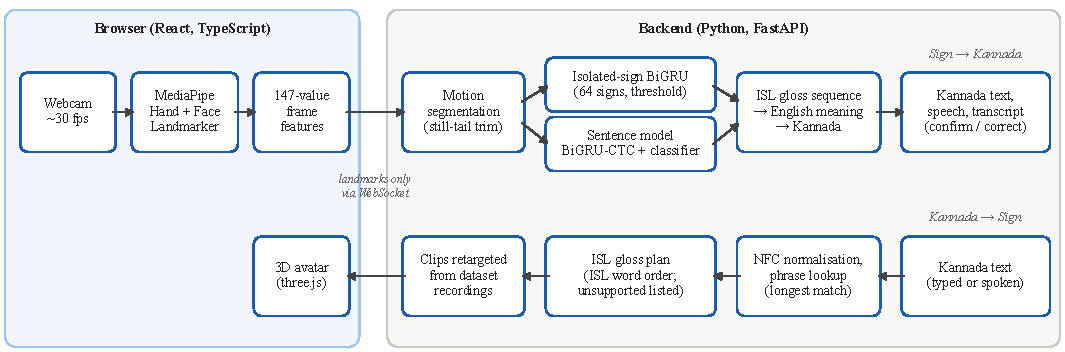
\includegraphics[width=\textwidth]{fig_architecture.pdf}
\caption{Kannada SignBridge architecture. Only landmark coordinates leave the browser. Top: sign to Kannada; bottom: Kannada to sign.}
\label{fig:arch}
\end{figure*}

\section{Methods}
\subsection{Landmark Features}
Each frame is encoded as a 147-dimensional vector (schema \texttt{hands-face-v2}). For each hand, 73 values describe the wrist-relative hand shape scaled by palm size (60), the position in the image (3), the position relative to the face (3), the finger direction and palm normal (6) and a presence flag (1); one value marks face visibility. A missing hand is flagged rather than filled with zeros. During dataset extraction, if the face detector fails on the full frame, it is re-run on an upper-centre crop of the original-resolution frame; this made face-relative features reliable for signs made near the face.

A segment of variable length is resampled to $T$ evenly spaced steps and complemented by wrist velocities and path lengths, giving an input of dimension
\begin{equation}
D = 147\,T + 6\,(T-1) + 2,
\end{equation}
i.e.\ $D=2{,}444$ for $T=16$ and $D=3{,}668$ for $T=24$ (current models). Each model stores its own $T$, so changing the default for new models never invalidates an existing one.

\subsection{Isolated-Sign Classifiers}
Three candidates are trained: multinomial logistic regression on standardised inputs; a bidirectional GRU \cite{cho2014gru,schuster1997bidirectional} with a per-frame linear embedding (96 units), 96 units per direction, mean and max pooling over time concatenated with global motion features, and a softmax output, trained with AdamW, class-weighted loss and early stopping; and an equal-weight probability ensemble of the two. Training data is augmented with five copies per sample using temporal cropping (up to 20\%), landmark jitter, position jitter and left-right mirroring (for left-handed signers and mirrored videos). The candidate with the highest signer-grouped cross-validation macro-F1 is selected; for the current model this was the BiGRU (0.368, against 0.357 for the ensemble and 0.305 for logistic regression).

\textit{Rejection threshold.} Every development video receives an out-of-fold prediction, and the confidence threshold that maximises the F1-score of accepted words is selected, where a non-sign predicted as a sign counts as an error. Predictions below the threshold are shown as ``uncertain'' with alternatives and are never added to the transcript automatically.

\subsection{Live Segmentation}
A sign starts when hand motion exceeds a threshold and ends after a stillness period, when the hands are lowered or leave the frame for 200\,ms, or after at most 4\,s. Training clips end with the hands moving, whereas live signers often hold the final position; the held-still frames at the end of a segment are therefore trimmed before classification. Replaying the 268 test videos through the live pipeline with the hold ending, this trimming raised the number of correctly recognised signs from 136 to 184.

\subsection{Continuous Sentence Recognition}
A two-layer BiGRU (128 units per direction) reads every second frame of a sentence and outputs, per time step, a distribution over 168 glosses plus the CTC blank \cite{graves2006ctc}. Separately, a logistic-regression sentence classifier operates on the sentence resampled to 32 steps. For each corpus sentence $s$ with gloss sequence $g_s$, the decoder scores
\begin{equation}
\mathrm{score}(s) = \log P_{\mathrm{CTC}}(g_s \mid X) + \lambda \log P_{\mathrm{cls}}(s \mid X),
\end{equation}
with $\lambda=1.0$ chosen on the validation round. The softmax of the scores gives a posterior; sentences with posterior below 0.5 (also chosen on validation) are shown as uncertain with the three best candidates. The sentence results in Section~VI refer to this decoder.

\subsection{Model Governance}
Every trained model is stored as a version with its metrics, its per-video test predictions and a status record. A new model becomes active only if (i) its held-out macro-F1 is at least 0.40, (ii) it is not worse than the active model by more than 0.02 on the test videos both share, and (iii) it passes a reload and live-pipeline smoke test; earlier versions remain available for rollback.

\section{Results}
\subsection{Isolated Signs}
Table~\ref{tab:iso} and Fig.~\ref{fig:results} summarise the development on the identical 268 held-out videos. Temporal modelling and face-crop extraction raised accuracy from 59.7\% to 72.4\%. The INCLUDE expansion then raised it to 79.9\%; on the 213 videos of the two unseen Amrita signers, the most demanding subset, accuracy rose from 67.1\% to 76.5\%. Paired on the same 268 videos, 34 videos became correct and 13 became wrong (exact McNemar $p=0.003$). The largest gains were for the signs that received new data, such as GREY, BLACK, BIRD, DOG, FATHER, FISH and BOY.

\begin{table}[t]
\caption{Isolated-sign accuracy (\%) on the same held-out videos}
\label{tab:iso}
\centering
\setlength{\tabcolsep}{4pt}
\begin{tabular}{@{}lrrrr@{}}
\toprule
Model (training videos) & All & Amrita & INCLUDE & Macro- \\
 & (268) & unseen (213) & test (55) & F1 \\
\midrule
LogReg baseline (1{,}290) & 59.7 & 54.5 & 80.0 & 0.591 \\
LogReg+BiGRU, $T{=}16$ (1{,}290) & 72.4 & 67.1 & 92.7 & 0.708 \\
LogReg+BiGRU, $T{=}24$ (1{,}290) & 72.0 & 67.1 & 90.9 & 0.707 \\
\textbf{BiGRU + INCLUDE (1{,}749)} & \textbf{79.9} & \textbf{76.5} & \textbf{92.7} & \textbf{0.800}$^{*}$ \\
\bottomrule
\multicolumn{5}{@{}l}{\footnotesize $^{*}$Macro-F1 on its full 314-video test set (accuracy 81.5\%).}
\end{tabular}
\end{table}

\begin{figure}[t]
\centering
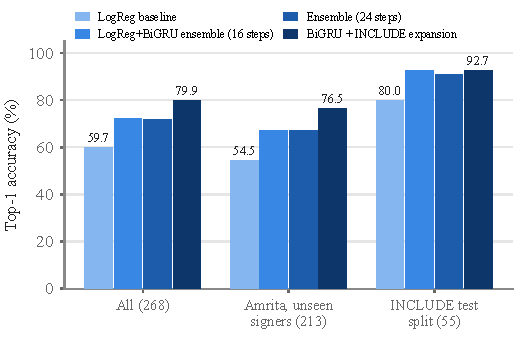
\includegraphics[width=\columnwidth]{fig_results.pdf}
\caption{Top-1 accuracy of successive models on the identical held-out videos.}
\label{fig:results}
\end{figure}

\textit{Streaming.} Replaying the 314 test videos back to back through the live pipeline (segmentation, threshold and duplicate suppression) gives a sign error rate of 0.274 (54 substitutions, 8 deletions and 24 insertions over 314 signs). The back end needs 1.4\,ms per frame on a laptop CPU.

\textit{Browser and training-time features.} Running eight dataset videos through the in-browser MediaPipe path and the offline Python path gave hand-presence agreement of 91.8--100\% and the same predicted label for seven of eight videos, confirming that live and training features match.

\textit{Rejected larger vocabulary.} Adding 79 further INCLUDE signs (144 classes, 3{,}182 training videos) reached 85.2\% on 210 INCLUDE test videos of the new signs, but lowered accuracy on the original signs from 81.5\% to 76.1\% and on unseen Amrita signers from 76.5\% to 70.9\%. The promotion gate rejected it. Because INCLUDE's official split reuses signers between training and test, the 85.2\% likely overestimates performance for new users.

\subsection{Continuous Sentences}
Table~\ref{tab:sent} compares decoders on the same networks and the 154 test videos of unseen recording rounds. The fused decoder reaches 29.2\% exact-sentence accuracy (chance is about 1\%) and the lowest gloss error rate. Of the 122 sentences shown with posterior of at least 0.5, 43 are correct; the other 32 videos are reported as uncertain. Retraining the same recipe with different random seeds gave 20.1--29.2\%, so differences of a few points between single runs are not meaningful. A candidate trained on cleaned data plus 187 additional unlisted videos scored 22.1\% and was rejected (McNemar $p=0.052$ in favour of the existing model).

\begin{table}[t]
\caption{Sentence decoders on 154 test videos of unseen rounds}
\label{tab:sent}
\centering
\begin{tabular}{@{}lrr@{}}
\toprule
Decoder & Sentence acc. (\%) & GER \\
\midrule
Sentence classifier only & 20.1 & 0.883 \\
CTC greedy path $\rightarrow$ nearest sentence & 18.2 & 0.742 \\
CTC likelihood of each sentence & 22.1 & 0.724 \\
\textbf{CTC likelihood + classifier (fused)} & \textbf{29.2} & \textbf{0.685} \\
\bottomrule
\end{tabular}
\end{table}

\section{Discussion and Limitations}
\textit{Recorded video is not live use.} All accuracies above are measured on recorded dataset videos of unseen signers. Live webcam accuracy depends on camera, lighting, distance and on whether the user signs the regional variant present in the training data (Kerala for Amrita SLR, Chennai for INCLUDE). The system therefore includes an evaluation-only recording mode and a live evaluation report with error attribution; these measurements are the next step and are not yet available. A reference page shows the dataset recordings of each sign so that users can see the variant the model was trained on.

\textit{Vocabulary and data.} With about 14--42 recordings per sign from few signers, adding classes reduced accuracy on existing ones, and the sentence model is restricted to the 101 corpus sentences, so it is not open-vocabulary sign language translation. Signs performed back to back without lowering the hands can merge into one segment.

\textit{Kannada and avatar.} Kannada wording received an AI-assisted check only, and avatar clips retargeted from 2-D landmarks are approximate; both require review by native Kannada speakers and ISL users before real use.

\section{Conclusion and Future Work}
Kannada SignBridge demonstrates a complete, privacy-preserving ISL--Kannada pipeline on a CPU-only laptop, with signer-independent evaluation and a governance process that prevents regressions from reaching users. Additional real ISL data was the most effective single improvement, raising unseen-signer accuracy from 67.1\% to 76.5\%. Future work comprises live webcam evaluation sessions, recordings from Karnataka signers to cover regional variants and to support a larger vocabulary, sentence-level training on larger ISL corpora such as iSign \cite{joshi2024isign}, and review of the Kannada output and avatar clips by the deaf community.

\section*{Acknowledgment}
The authors thank the creators of the Amrita SLR, INCLUDE and ISL-CSLTR datasets and the signers who recorded them.

\begin{thebibliography}{00}
\bibitem{li2020wlasl} D. Li, C. Rodriguez, X. Yu, and H. Li, ``Word-level deep sign language recognition from video: A new large-scale dataset and methods comparison,'' in \textit{Proc. IEEE/CVF Winter Conf. Applications of Computer Vision (WACV)}, 2020, pp. 1459--1469.
\bibitem{joze2019msasl} H. R. Vaezi Joze and O. Koller, ``MS-ASL: A large-scale data set and benchmark for understanding American Sign Language,'' in \textit{Proc. British Machine Vision Conf. (BMVC)}, 2019.
\bibitem{koller2015continuous} O. Koller, J. Forster, and H. Ney, ``Continuous sign language recognition: Towards large vocabulary statistical recognition systems handling multiple signers,'' \textit{Computer Vision and Image Understanding}, vol. 141, pp. 108--125, 2015.
\bibitem{camgoz2018neural} N. C. Camgoz, S. Hadfield, O. Koller, H. Ney, and R. Bowden, ``Neural sign language translation,'' in \textit{Proc. IEEE/CVF Conf. Computer Vision and Pattern Recognition (CVPR)}, 2018, pp. 7784--7793.
\bibitem{sridhar2020include} A. Sridhar, R. G. Ganesan, P. Kumar, and M. Khapra, ``INCLUDE: A large scale dataset for Indian Sign Language recognition,'' in \textit{Proc. 28th ACM Int. Conf. Multimedia}, 2020, pp. 1366--1375, doi: 10.1145/3394171.3413528.
\bibitem{elakkiya2021csltr} R. Elakkiya and B. Natarajan, ``ISL-CSLTR: Indian Sign Language dataset for continuous sign language translation and recognition,'' Mendeley Data, V1, 2021, doi: 10.17632/kcmpdxky7p.1.
\bibitem{amrita2023} R. Sasidharan, M. Rashmi, K. S. Nair, N. S. Heera Krishna, K. Muraleedharan, N. G. Bellamkonda, S. M. Rao, S. Avvari, P. B. Prakash, and D. T. Rao, ``Amrita SLR -- Real time ISL dataset,'' Mendeley Data, V1, 2025, doi: 10.17632/dtg9s785v8.1.
\bibitem{joshi2023isltranslate} A. Joshi, S. Agrawal, and A. Modi, ``ISLTranslate: Dataset for translating Indian Sign Language,'' in \textit{Findings of the Association for Computational Linguistics: ACL 2023}, 2023.
\bibitem{joshi2024isign} A. Joshi, R. Mohanty, M. Kanakanti, A. Mangla, S. Choudhary, M. Barbate, and A. Modi, ``iSign: A benchmark for Indian Sign Language processing,'' in \textit{Findings of the Association for Computational Linguistics: ACL 2024}, 2024.
\bibitem{lugaresi2019mediapipe} C. Lugaresi \textit{et al.}, ``MediaPipe: A framework for building perception pipelines,'' arXiv:1906.08172, 2019.
\bibitem{zhang2020mediapipehands} F. Zhang \textit{et al.}, ``MediaPipe Hands: On-device real-time hand tracking,'' arXiv:2006.10214, 2020.
\bibitem{jiang2021skeleton} S. Jiang, B. Sun, L. Wang, Y. Bai, K. Li, and Y. Fu, ``Skeleton aware multi-modal sign language recognition,'' in \textit{Proc. IEEE/CVF Conf. Computer Vision and Pattern Recognition Workshops (CVPRW)}, 2021, pp. 3413--3423.
\bibitem{cho2014gru} K. Cho \textit{et al.}, ``Learning phrase representations using RNN encoder--decoder for statistical machine translation,'' in \textit{Proc. Conf. Empirical Methods in Natural Language Processing (EMNLP)}, 2014, pp. 1724--1734.
\bibitem{schuster1997bidirectional} M. Schuster and K. K. Paliwal, ``Bidirectional recurrent neural networks,'' \textit{IEEE Trans. Signal Processing}, vol. 45, no. 11, pp. 2673--2681, 1997.
\bibitem{graves2006ctc} A. Graves, S. Fern\'andez, F. Gomez, and J. Schmidhuber, ``Connectionist temporal classification: Labelling unsegmented sequence data with recurrent neural networks,'' in \textit{Proc. 23rd Int. Conf. Machine Learning (ICML)}, 2006, pp. 369--376.
\bibitem{mcnemar1947} Q. McNemar, ``Note on the sampling error of the difference between correlated proportions or percentages,'' \textit{Psychometrika}, vol. 12, no. 2, pp. 153--157, 1947.
\end{thebibliography}

\end{document}
